\section{Setup and Procedure}
To determine the rubidium absorption spectrum with a diode laser it is important to make different premeasurements.
For each measurement it is necessary to use another setup. For all setups it is advisable to darken the room.

\noindent
In the following each setup aim and the setup itself will be explained.

\subsection{Threshold current}
First of all it is important to register the threshold current since below it the diode only works as a LED and 
only above as a laser.
The setup for this is really simple. The laser is connected to a powersource where the current can be changed. 
In front of the laser is a businesscard holder placed with a card which is converting infrared light into 
visible light. 
Since the laser is operating in the infrared spectrum this card is necessary to make the light visible.
A camera is directed at the card too. The setup is sketched in figure \ref{fig:th}.

\begin{figure}[H]
	\centering
	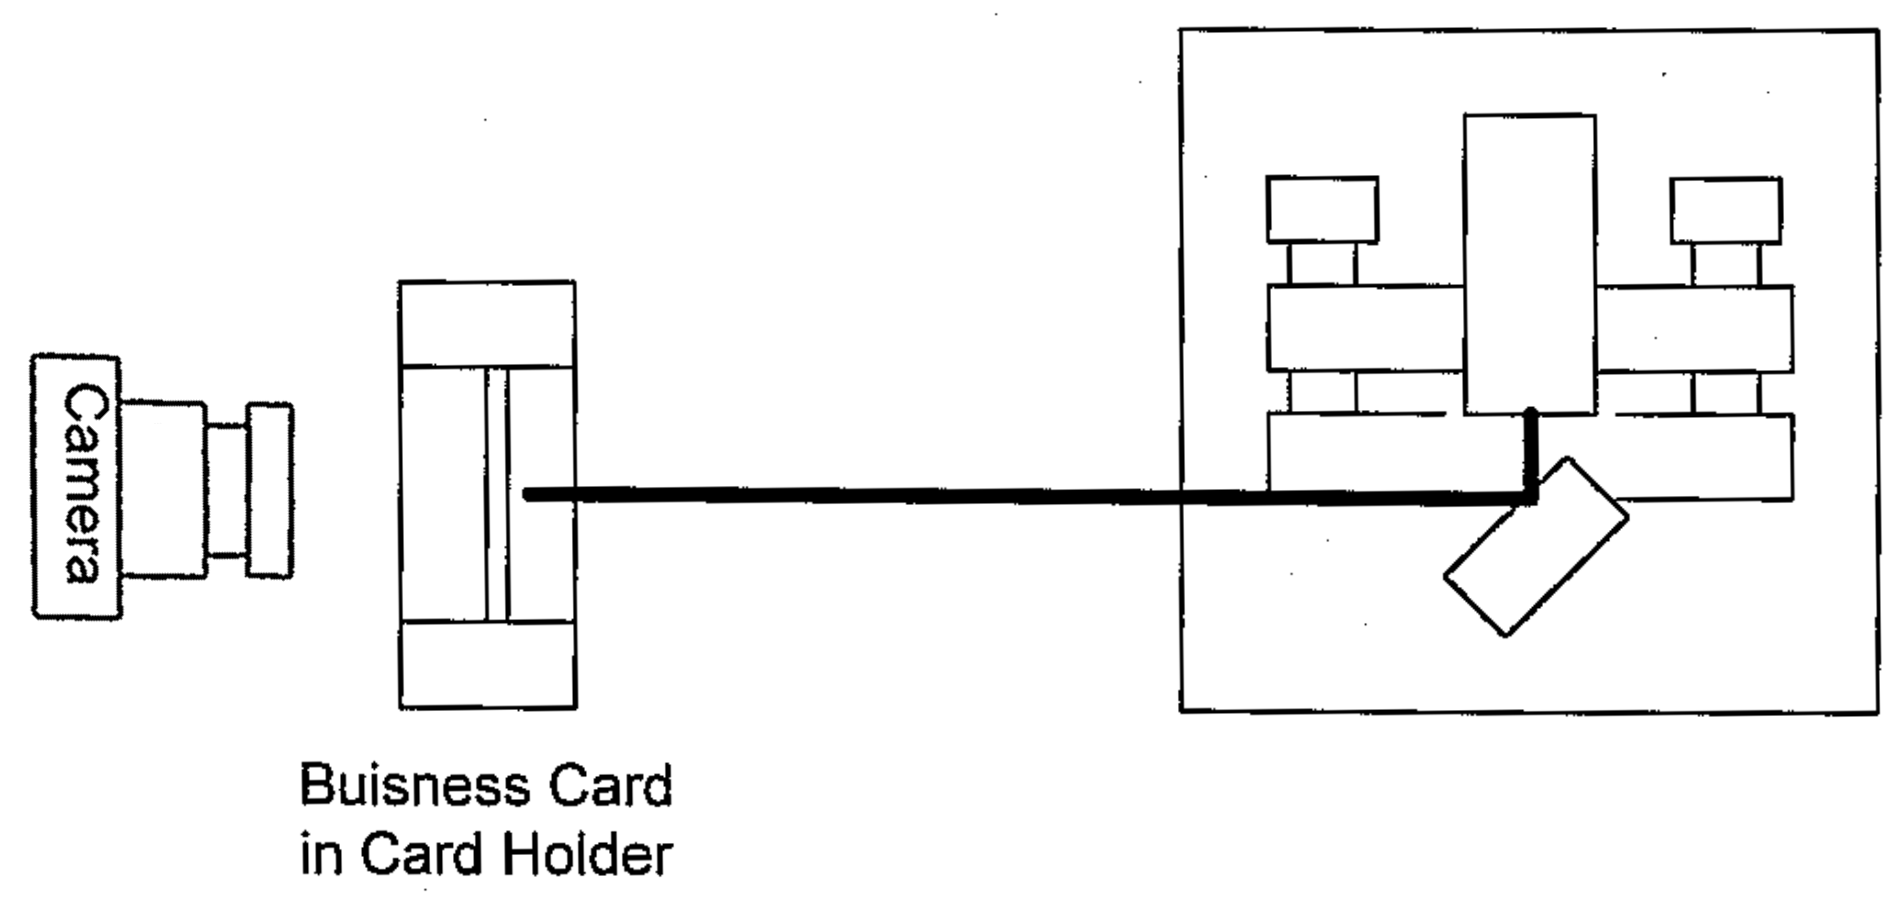
\includegraphics[width=\textwidth]{setup_threshold.png}
	\caption{Sketch of the setup for finding the threshold. \cite{V60}}
	\label{fig:th}
\end{figure}

\noindent
By changing the current the threshold can be found. The threshold current is at the transition point where the light spot
becomes significantly brighter and begins to crimble in the video of the camera.

\subsection{Rubidium fluorescence}
The next setup is build to see the fluorescence of the Rubidium. The businesscard holder is replaced by a chamber
filled with Rubidium. 
The laserlight is directly directed into the chamber. On the right hand side of the chamber is a cutout where
a camera is placed to observe the fluorescence light. The setup is sketched in figure \ref{fig:fl}. Also
 the ramp generator and piezo controller are wired as shown in figure \ref{fig:rg}.

\begin{figure}[H]
	\centering
	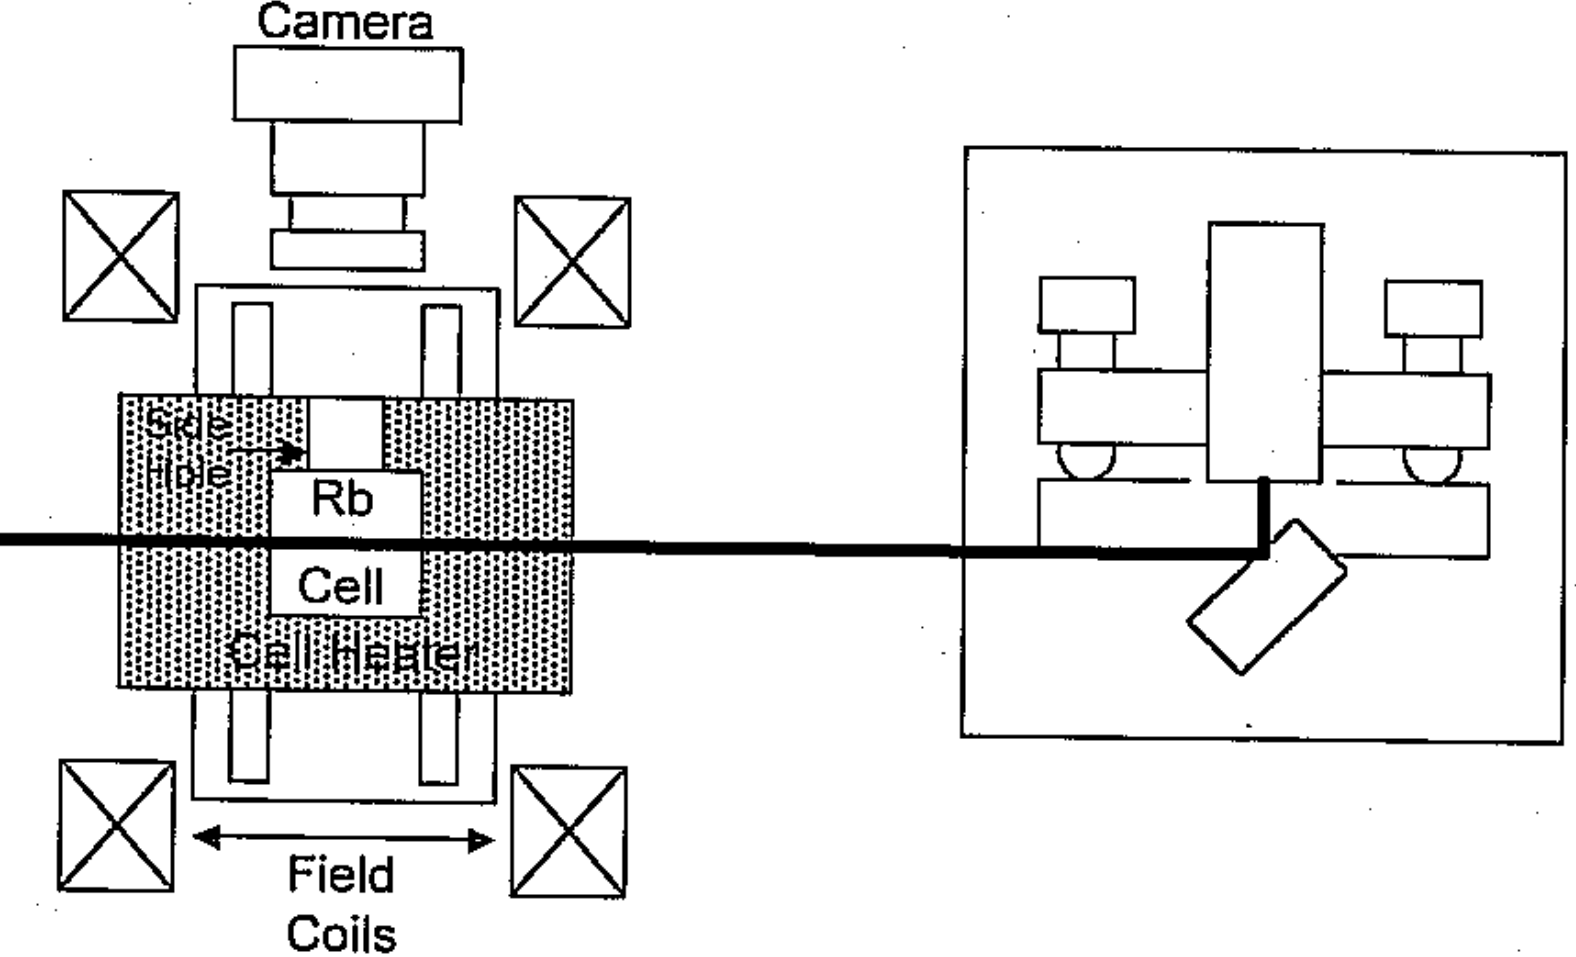
\includegraphics[width=\textwidth]{setup_fluorescence.png}
	\caption{Sketch of the setup to observe fluorescence light. \cite{V60}}
	\label{fig:fl}
\end{figure}

\noindent
The current gets set to the threshold and then slowly increased until a light beam is visible in the video of the 
camera.

\begin{figure}[H]
	\centering
	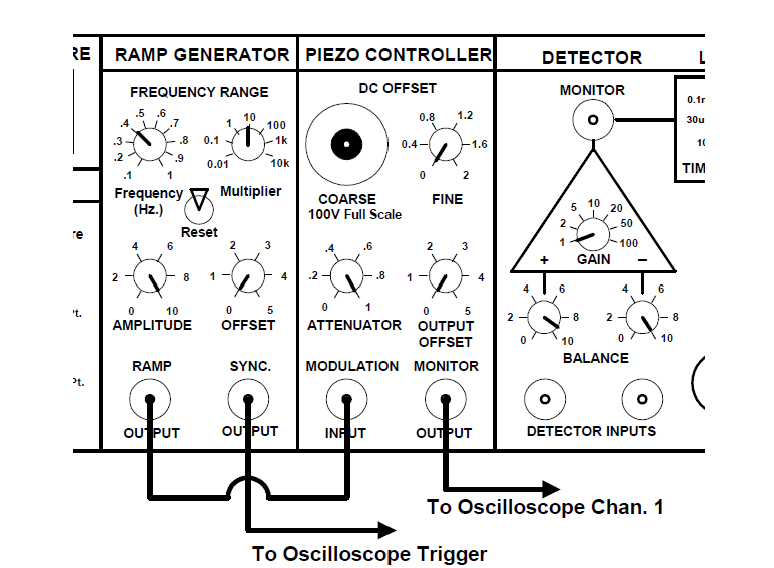
\includegraphics[width=\textwidth]{setup.png}
	\caption{Wiring of the ramp generator and the piezo controller. \cite{V60}}
	\label{fig:rg}
\end{figure}

\noindent
It is also important to note that the laser has two knobs. With the upper one the verticle angle of the grating can
be changed and with the lower one it is possible to change the horizontal angle.

\begin{figure}[H]
	\centering
	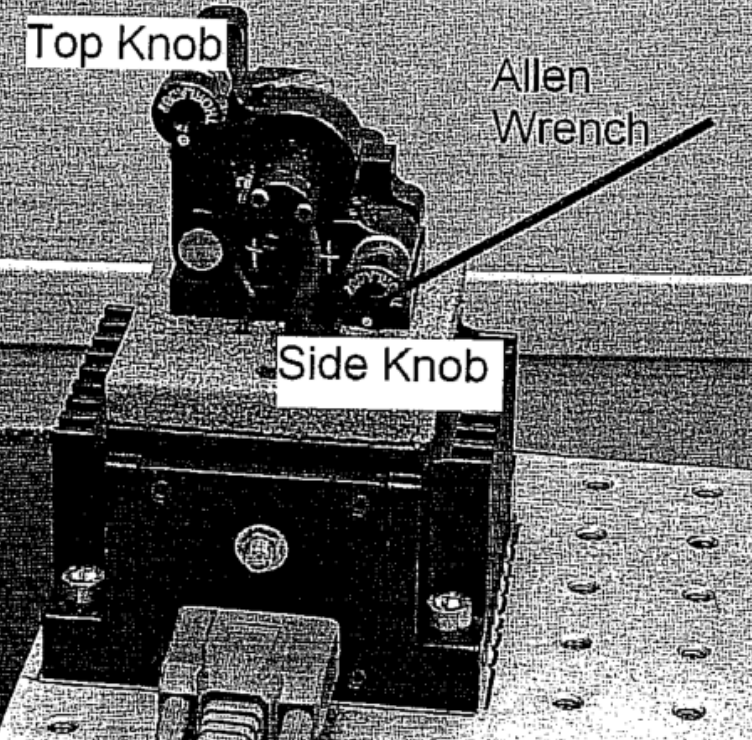
\includegraphics[width=\textwidth]{laser.png}
	\caption{Picture of the laser with the knobs. \cite{V60}}
	\end{figure}

\subsection{Rubidium absorption spectrum}
The final setup is to detect the absorption spectrum of Rubidium. For this 2 photodetectors, a half-transparent
mirror (reflects half of the light), a glas nd-filter and a gelatin nd-filter is added. The way they are added is 
shown in figure \ref{fig:sub} and the wiring is shown in figure \ref{fig:set1}.

\begin{figure}[H]
	\centering
	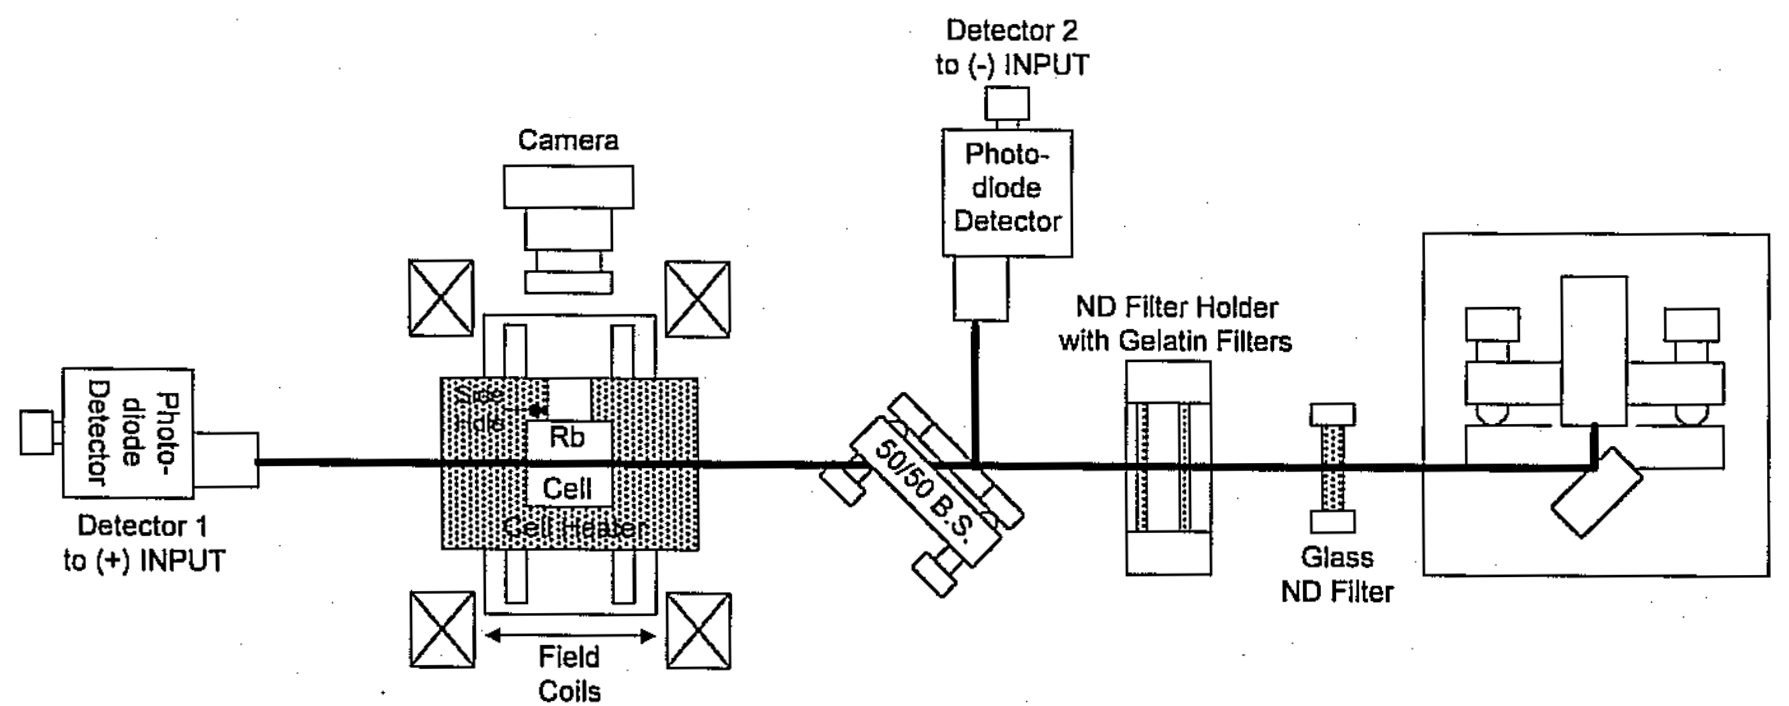
\includegraphics[width=\textwidth]{setup_substraction.png}
	\caption{Setup to observe the Rubidium fluorescence. \cite{V60}}
	\label{fig:sub}
\end{figure}

\begin{figure}[H]
	\centering
	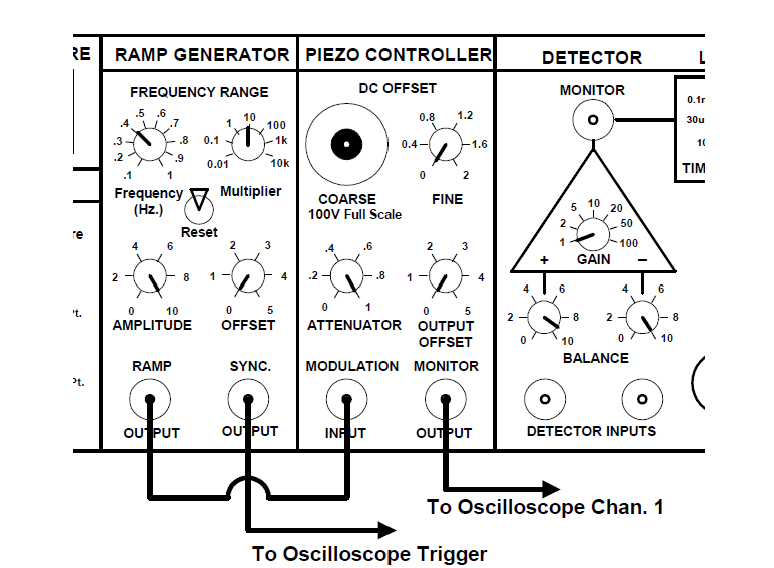
\includegraphics[width=\textwidth]{setup1.png}
	\caption{Wiring of the control element to observe the Rubidium fluorescence. \cite{V60}}
	\label{fig:set1}
\end{figure}

\noindent
The first photodetector is necessary to detect the out going light beam, the second one is needed to flatten
the curve of the detected spectrum, since it is proportional to the current created by the ramp generator and
piezo controller. 

\noindent
The filter are needed because the photodetectors get easily overloaded by the high energy of the laser beam.
The spectrum of interest can be seen in the oscilloscope.




